\section{\textbf{The Simulation Environment}} \label{sec:Environment}

	Multiple applications that require verification and evaluation have become dependent of expensive resources, which makes their development a delicate matter. Examples of systems whose tests involve costly supplies are medical education~\cite{MEDIC}, the aviation industry~\cite{AIR} and automotive research and development~\cite{AUTR}; because naturally no company or enterprise has expendable numbers of bodies for tests, or airplanes and cars to crash in order to safe-proof and improve. In these conditions computer simulations arise, virtually reproducing the environments of the said and of other important applications so that their testbeds reduce the need of the scarce resources related to them.
	
	Many other reasons justify the use of virtual simulations, varying from one application to another, and, because of this, countless companies are incorporating them in their educational and training process~\cite{Simulation}~\cite{Operator}. A few number of reasons why a simulation was used in this work:
	
	\begin{itemize}
		
		\item managing control operations;
		
		\item planning actions;
		
		\item understanding a problem and finding out how to react to it;
		
		\item training and learning through experimentation.
		
	\end{itemize}
	
	Simulations represent just an approximated model of the systems they try to imitate, but in most cases the effects of the estimates adopted in the attempt to do this do not come to the point that the model becomes invalid. Similarly, car racing simulations also incorporate flawed modeling - regarding friction, gravity, trajectory lines, and so on - but resorting to them may save some spare parts that would most likely be jeopardized in real-life tests. So, new studies, new researches and new automation methods might be evaluated through simulations and avoid costs in the development process.
	
\subsection{TORCS} \label{subsec:TORCS}

	The Open Racing Car Simulator (TORCS) is a platform that is renowned for its highly credible physics modeling engine and yet user-friendly interface for car racing simulations~\cite{TORCS}. It is a modern, multi-player and multi-agent car simulator; it also is an interface that is widely used for benchmarking AI~\cite{2009} due its high degree of modularity and portability, concerning multi-platform environments and support to the programming languages C and C++. Artificially intelligent agents can be developed as modules inside TORCS where there are many possible levels of abstraction. For example, at the car level, there is an intelligent control system for each car component; at the driver level, mid-level control systems for complex driving agents could be implemented using the partial simulation information given by a low-level API provided by TORCS.

	The TORCS engine~\cite{SIMUTORCS} uses a discrete-time simulation, whose discretization is set to approximately 0.002s of simulation time, and engine solves differential equations using \"{E}uler method, and all basic elements of the vehicular dynamics are handled, which are:

	\begin{itemize}
		
		\item basic properties of the vehicular system;
		
		\item mechanical details;
		
		\item dynamic and static friction;
		
		\item aerodynamic model.
		
	\end{itemize}

	Mass, rotational inertia of the car, engine, wheels, and other components, are included in the model of the vehicular system; while the types of different suspension, links, and differentials are done so in the mechanical model. The profiles for different ground types with both dynamic and static friction are also included; this way, the aerodynamics modeling includes slipstreaming and ground effects, that vary from one profile to another. Nevertheless, the simulation engine can be replaced or easily modified as a result of the modularity supplied by TORCS. The interface with this platform occurs by means of a sensor-based interaction system in which the developer is able to interpret received parameters of the car - such as speed in X, Y and even Z axes - and control the car through programming its actuators, some of which are acceleration and steering.
	
	Another credibility factor for this platform is its non-punctual cars that interact with each other in the races by a life-like collision system. Still, TORCS is still a simulator, and its limitations, along with the defined racing environment and the modeled car, are more than likely to affect any results obtained. This is an inherited characteristic of any real-life problem simulation, what in academia is denominated \emph{reality gap}~\cite{RG}, and it stems from the simplifications made concerning the car models, the technical features of the tracks, and so forth.
	
	The SCRC interface occurs in a way that TORCS allows the controller to have a full view of the environment including its exact location inside the track, the geometry and friction and also the exact location of all the other cars. In order to separate the controller logic from the simulator, the SCR interface was designed~\cite{2009}. This interface limits the information received by the controller, and the communication between this championship and TORCS is made through a client-server interface, with each player receiving information from the server regarding the sensors of the car, and in return providing actuator values that determine how the controller is supposed to drive the car.

\subsection{The SCR Championship} \label{subsec:SCRC}

	The Simulated Car Racing Championship (SCRC) is an example of a well-known competition which utilizes TORCS as interface~\cite{SCR}. Being an event joining three competitions held at major scientific conferences, such as \emph{IEEE Congress on Evolutionary Computation}~\footnote{http://www.cec2015.org/}, \emph{Genetic and Evolutionary Computation Conference}~\footnote{http://www.sigevo.org/gecco-2015/} and \emph{IEEE Conference on Computational Intelligence and Games}~\footnote{http://www.ieee-cig.org/}, it is an accepted metric of evaluation in the fields of Evolutionary Computation and Computational Intelligence regarding games in general.

   	\begin{figure}[h]
   		
		\centering
		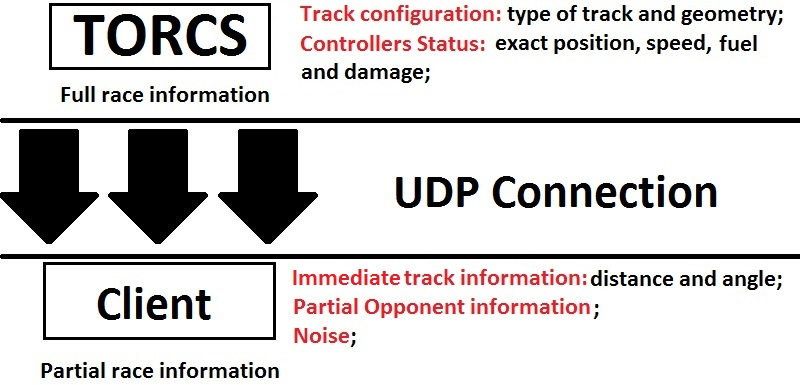
\includegraphics[width=250pt]{Figure1.jpg}
		\caption{Available data inside TORCS becoming data accessible to the client}
		\label{Fig:Comm}
		
	\end{figure}

	Race tracks are categorized into \emph{Road}, \emph{Dirt} and \emph{Oval} inside TORCS. The races from the SCRC take place in track types decided by the organization of the championship, information which is not provided to the participants and that may incorporate maps that are unknown to them. The competition adopts a structure that gathers a \textit{Warm-up} stage, a \textit{Qualifier} stage and a \textit{Final} race. Noise can be introduced in the sensors, option that is present during the actual competition. The complete sensorial input information and all the details concerning the race stages and types are presented at the Simulated Car Racing Championship Competition Software Manual~\cite{SCRC}.
	
	The reason why TORCS presents itself as a satisfactory AI benchmark, in combination with SCRC, is because even	though there are multiple possibilities on how the sensorial input received from the server can be translated into the behavior of the actuators, they can all be compared in a race, which has a robust and steady scoring and evaluational system. In other words, there are many different approaches concerning how to teach the racer encoded by the developers to drive in a racing competition only with the information given by the sensors, and the metric to that issue is the performance on the race itself.

\subsection{Related Works and State of the Art} \label{subsec:Related}
	
	It is very common among some of the SCRC awarded controllers the incorporation of machine learning in their driving methods, along with other evolving techniques using artificial intelligence~\cite{2009}. As the nature of the problematic presented comprises evolution by experience, learning procedures tend to enhance performance and competitiveness. Essentially, there are two ways of evolving learning solutions: Online Learning and Offline Learning.

	According to Tom Mitchel in \emph{Machine Learning}~\cite{Mitcchel:ML}:

	\begin{quotation} \itshape

		``Systems that learn by moving about the real environment and observing the results are typically called online systems, whereas those that earn solely by simulating actions within an internal model are called ofline systems.''
	
	\end{quotation}

	The current champion of the SCR Championship is the controller \emph{Mr. Racer}~\cite{MrRacer}, and it has proven to be the State of the Art by winning the last three competitions that happened from 2011 to 2013. The authors of this implementation employ several heuristics and black-box optimization methods in order to reproduce the mechanisms to which human racing drivers resort, doing so by means of a modular structure. \emph{Mr. Racer} uses a Covariance Matrix Adaptation Evolution Strategy (CMA-ES), to evolve parameters offline.
	
	According to the founders of the competition~\cite{SCRC} and the authors of \emph{Mr. Racer} themselves, \emph{AUTOPIA}~\cite{AUTOPIA} is another competitive controller, with the potential to even be the best one available. \emph{AUTOPIA} implements a modular Fuzzy Architecture, whose division contains gear, steering and speed control; and it is optimized by means of a genetic algorithm for Offline Learning, and by means of landmarking the lane exit points for further speed reduction for Online Learning.
	
	These and other controller exemplifications~\cite{SCRC} served as criteria for the analysis and development of the approach presented in this paper. Elements incorporated and adapted from them feature modularity, Offline Learning through genetic algorithms, Online Learning through landmarking and choosing sets of parameters for different categories of tracks, etc.
	
